

Model-Driven Software Development focuses on managing abstract models representing the conceptual level of the solution space. These models are generally represented as various artifacts, corresponding to different languages and using different representations. But models are rarely executable and/or lack the required level of expressiveness or performance to be exploited directly in production. Thus, the solution they offer is often implemented by using code generators that produce a representation of the solution in a target programming language or framework\cite{stahl2006model}. The underlying semantics of the code to be executed is generally encoded in those code generators and can be inlined or implicitly defined by the code generation process, or may be sometimes explicit to the code generation. Figure \ref{fig:ClassicalVision} shows the classical vision for Model-Driven Engineering.

This approach, model first, then generation, raises two major issues. First, it creates an important gap between the conceptual level (the model) and the source code, where semantics may be totally hidden or implicit. Second, the synchronization of the pair models-code in a co-evolution scenario where model and source code may evolve independently (and often by different actors, e.g., architect and developer) becomes hard to maintain.

Round-trip mechanisms are commonly used to overcome those difficulties, but they are difficult to use and to maintain. Indeed, the model/code co-evolution problem remains an open subject in the software engineering research community and, consequently, software development projects often abandon the idea of maintaining the synchronization between model and source code during development process. In that context, the model is developed at the early stages of development process, used mainly to prototype software application. Then, it may be manually reviewed back at the end of development process, for documentation purposes.

\begin{figure}
    \centering
    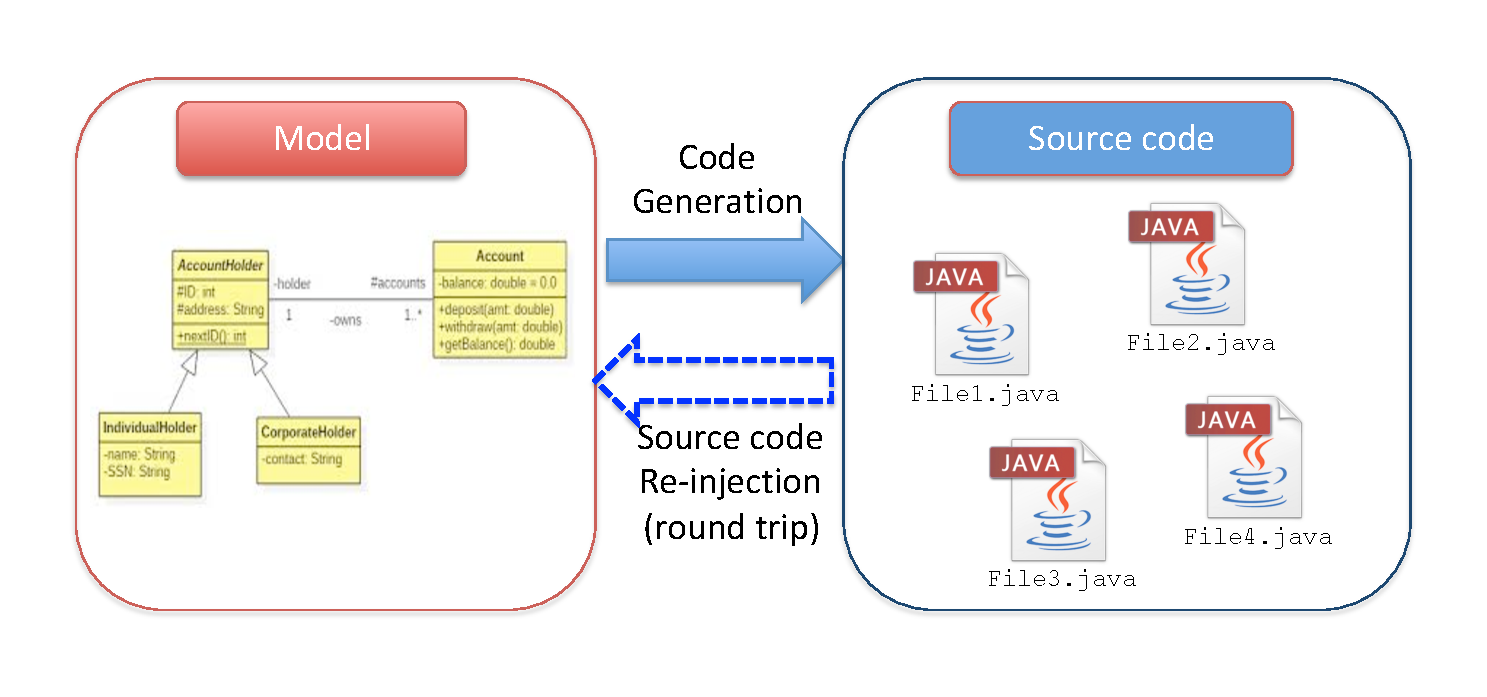
\includegraphics[width=1.0\columnwidth]{ClassicalVision.pdf}
    \caption{Classical vision for Model-Driven Engineering}
    \label{fig:ClassicalVision}
\end{figure}

Conversely, we propose a shift in the modeling paradigm in which models and code are developed together and at the same time in what we call a continuous modeling process. The PAMELA framework supports this paradigm shift by providing the means to: 1) annotate Java code with model-based annotations; and 2) interpret these annotations at runtime.

%\todo[inline]{In some sense we are loosing some of the advantages of modeling, aren't we? But let's see what reviewers say.}

% On peut éventuellement supprimer ce paragraphe
The rest of the paper is organized as follows. Section \ref{sec:pamproc} describes our approach and its associated development process. Section \ref{sec:architecture} presents the main building blocks of the PAMELA framework together with an illustrative example. Implementation details are discussed in Section \ref{sec:implementation}, followed by a description of industrial experimentation and validation cases in Section \ref{sec:validation}. We end the paper in Section \ref{sec:related} by discussing related work.


